\documentclass[xcolor=table]{beamer}
\usetheme{default}
\definecolor{darkscarlet}{rgb}{0.34, 0.01, 0.1}
\usecolortheme{default}
\usecolortheme[named=darkscarlet]{structure}
\setbeamercolor{title}{bg=white, fg=darkscarlet}
\definecolor{cerise}{rgb}{0.87, 0.19, 0.39}
\hypersetup{colorlinks=TRUE,linkcolor=cerise,urlcolor=cerise, citecolor=cerise}

% nummering

\setbeamertemplate{caption}[numbered]

% taal

% tekens
\usepackage{fontspec}
\usefonttheme{serif}
\setmainfont[BoldFont=brillb.ttf, ItalicFont=brilli.ttf, BoldItalicFont=brillbi.ttf]{brill.ttf}

% tekst doorstrepen, kennelijk heb je daar een apart pakket voor nodig

\usepackage[normalem]{ulem}

% plaatjes

\usepackage{graphicx}
\usepackage{subfig}

% tabellen

\usepackage{multirow}

% voorbeelden

\usepackage{philex}
\usepackage{forest}

% glossen

\usepackage{leipzig}
\newleipzig{hab}{hab}{habitual}
\newleipzig{aor}{aor}{aorist}
\makeglossaries

% bibliography

\usepackage[backend=biber,
        bibstyle=biblatex-sp-unified,
        citestyle=sp-authoryear-comp,
        doi=false,
        maxcitenames=3,
        maxbibnames=99]{biblatex}
\addbibresource{bibliography.bib}


% custom footline

\setbeamerfont{footline}{size=\fontsize{20}{20}\selectfont}

\newcommand{\Ffootline}{\footnotesize
\insertsection
\hfill
\href{https://github.com/agricolamz/2020.03.24_NIS_dictionaries}{github/agricolamz/2020.03.24\_NIS\_dictionaries}
\hfill
\insertframenumber/\inserttotalframenumber} 

% custom footline deel 2

\setbeamertemplate{footline}{%
\usebeamerfont{structure}
\begin{beamercolorbox}[wd=\paperwidth,ht=2.25ex,dp=1ex]{title in head/foot}%
\Tiny\hspace*{4mm} \Ffootline \hspace{4mm}
\end{beamercolorbox}}

% navigatiesymbolen uitzetten

\beamertemplatenavigationsymbolsempty
 
 
% titelpagina 

\title{Phonological and morphological variation in Botlikh: \\ Comparing two dictionaries}
\author{George Moroz, Chiara Naccarato, Samira Verhees \\
Linguistic Convergence Laboratory, NRU HSE}
\date{24.03.2020}

% links

\usepackage{hyperref}

%\newcommand\pro{\item[$+$]}
%\newcommand\con{\item[$-$]}

% ž š šč č ` 

\begin{document}

\begin{frame}
\titlepage
\end{frame}

\section{Introduction}
\begin{frame}{Botlikh}
    \begin{itemize}
        \item Botlikh < Andic < Avar-Andic-Tsezic < East Caucasian
        \item Spoken by \textasciitilde{}5,000-8,000 speakers
        \item Three villages in the Botlikh district of the Republic of Daghestan: Botlikh, Miarso, and Ashino
        \item Unwritten and mostly spoken at home; the Cyrillic script of Avar functions as an ad hoc writing system on social media
        \item Evaluated as ``threatened'' by Ethnologue \citep{simonsfenning2018}, but many children still speak the language and attitudes are positive
        \item Heavy influence from Avar and Russian 
    \end{itemize}
\end{frame}

\begin{frame}{Botlikh}
\begin{figure}[h]
\centering
\fbox{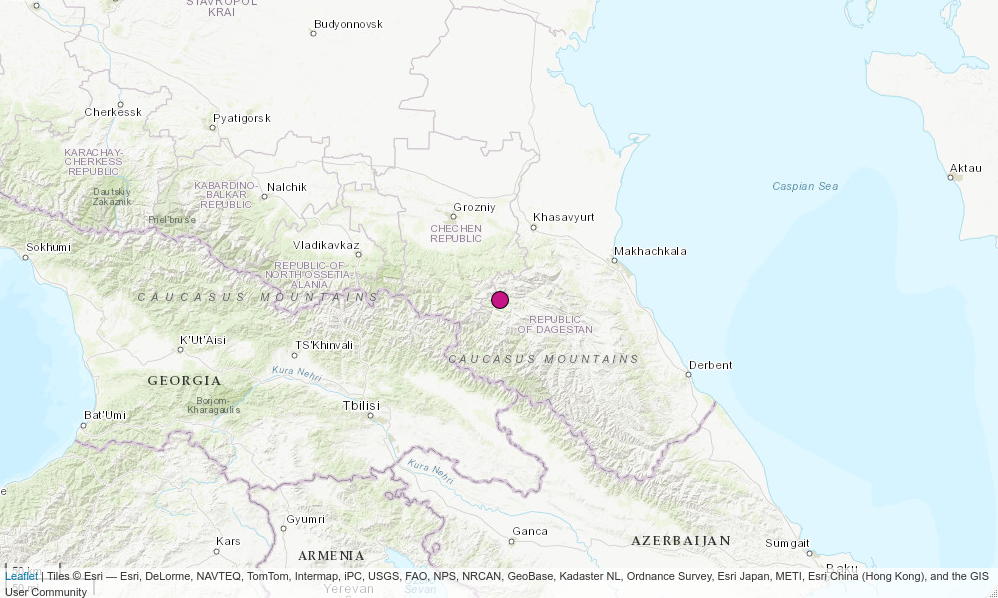
\includegraphics[scale=0.4]{images/globalmap.png}}
\caption{Botlikh on the map}
\end{figure}
\end{frame}

\begin{frame}{Botlikh literature}
\begin{itemize}
    \item One full reference grammar in Georgian \citep{gudava1962}
    \item Several short sketches mostly based on information contained in the grammar by Togo E. Gudava: \citep{gudava1967, azaev2000, saidova2001, magomedbekova2001, xalidova2017, alekseevverhees}
    \item Several works on the lexicon and word formation \citep{azaev1975, sulejmanova2013, alekseev2016}
    \item In general poorly described compared to other Andic languages like Godoberi or Bagvalal, BUT two Botlikh-Russian dictionaries are available to date \citep{saidovaabusov2012, alekseev2019}
\end{itemize}
\end{frame}

\begin{frame}{Two dictionaries}
\begin{figure}[h]
\begin{subfigure}
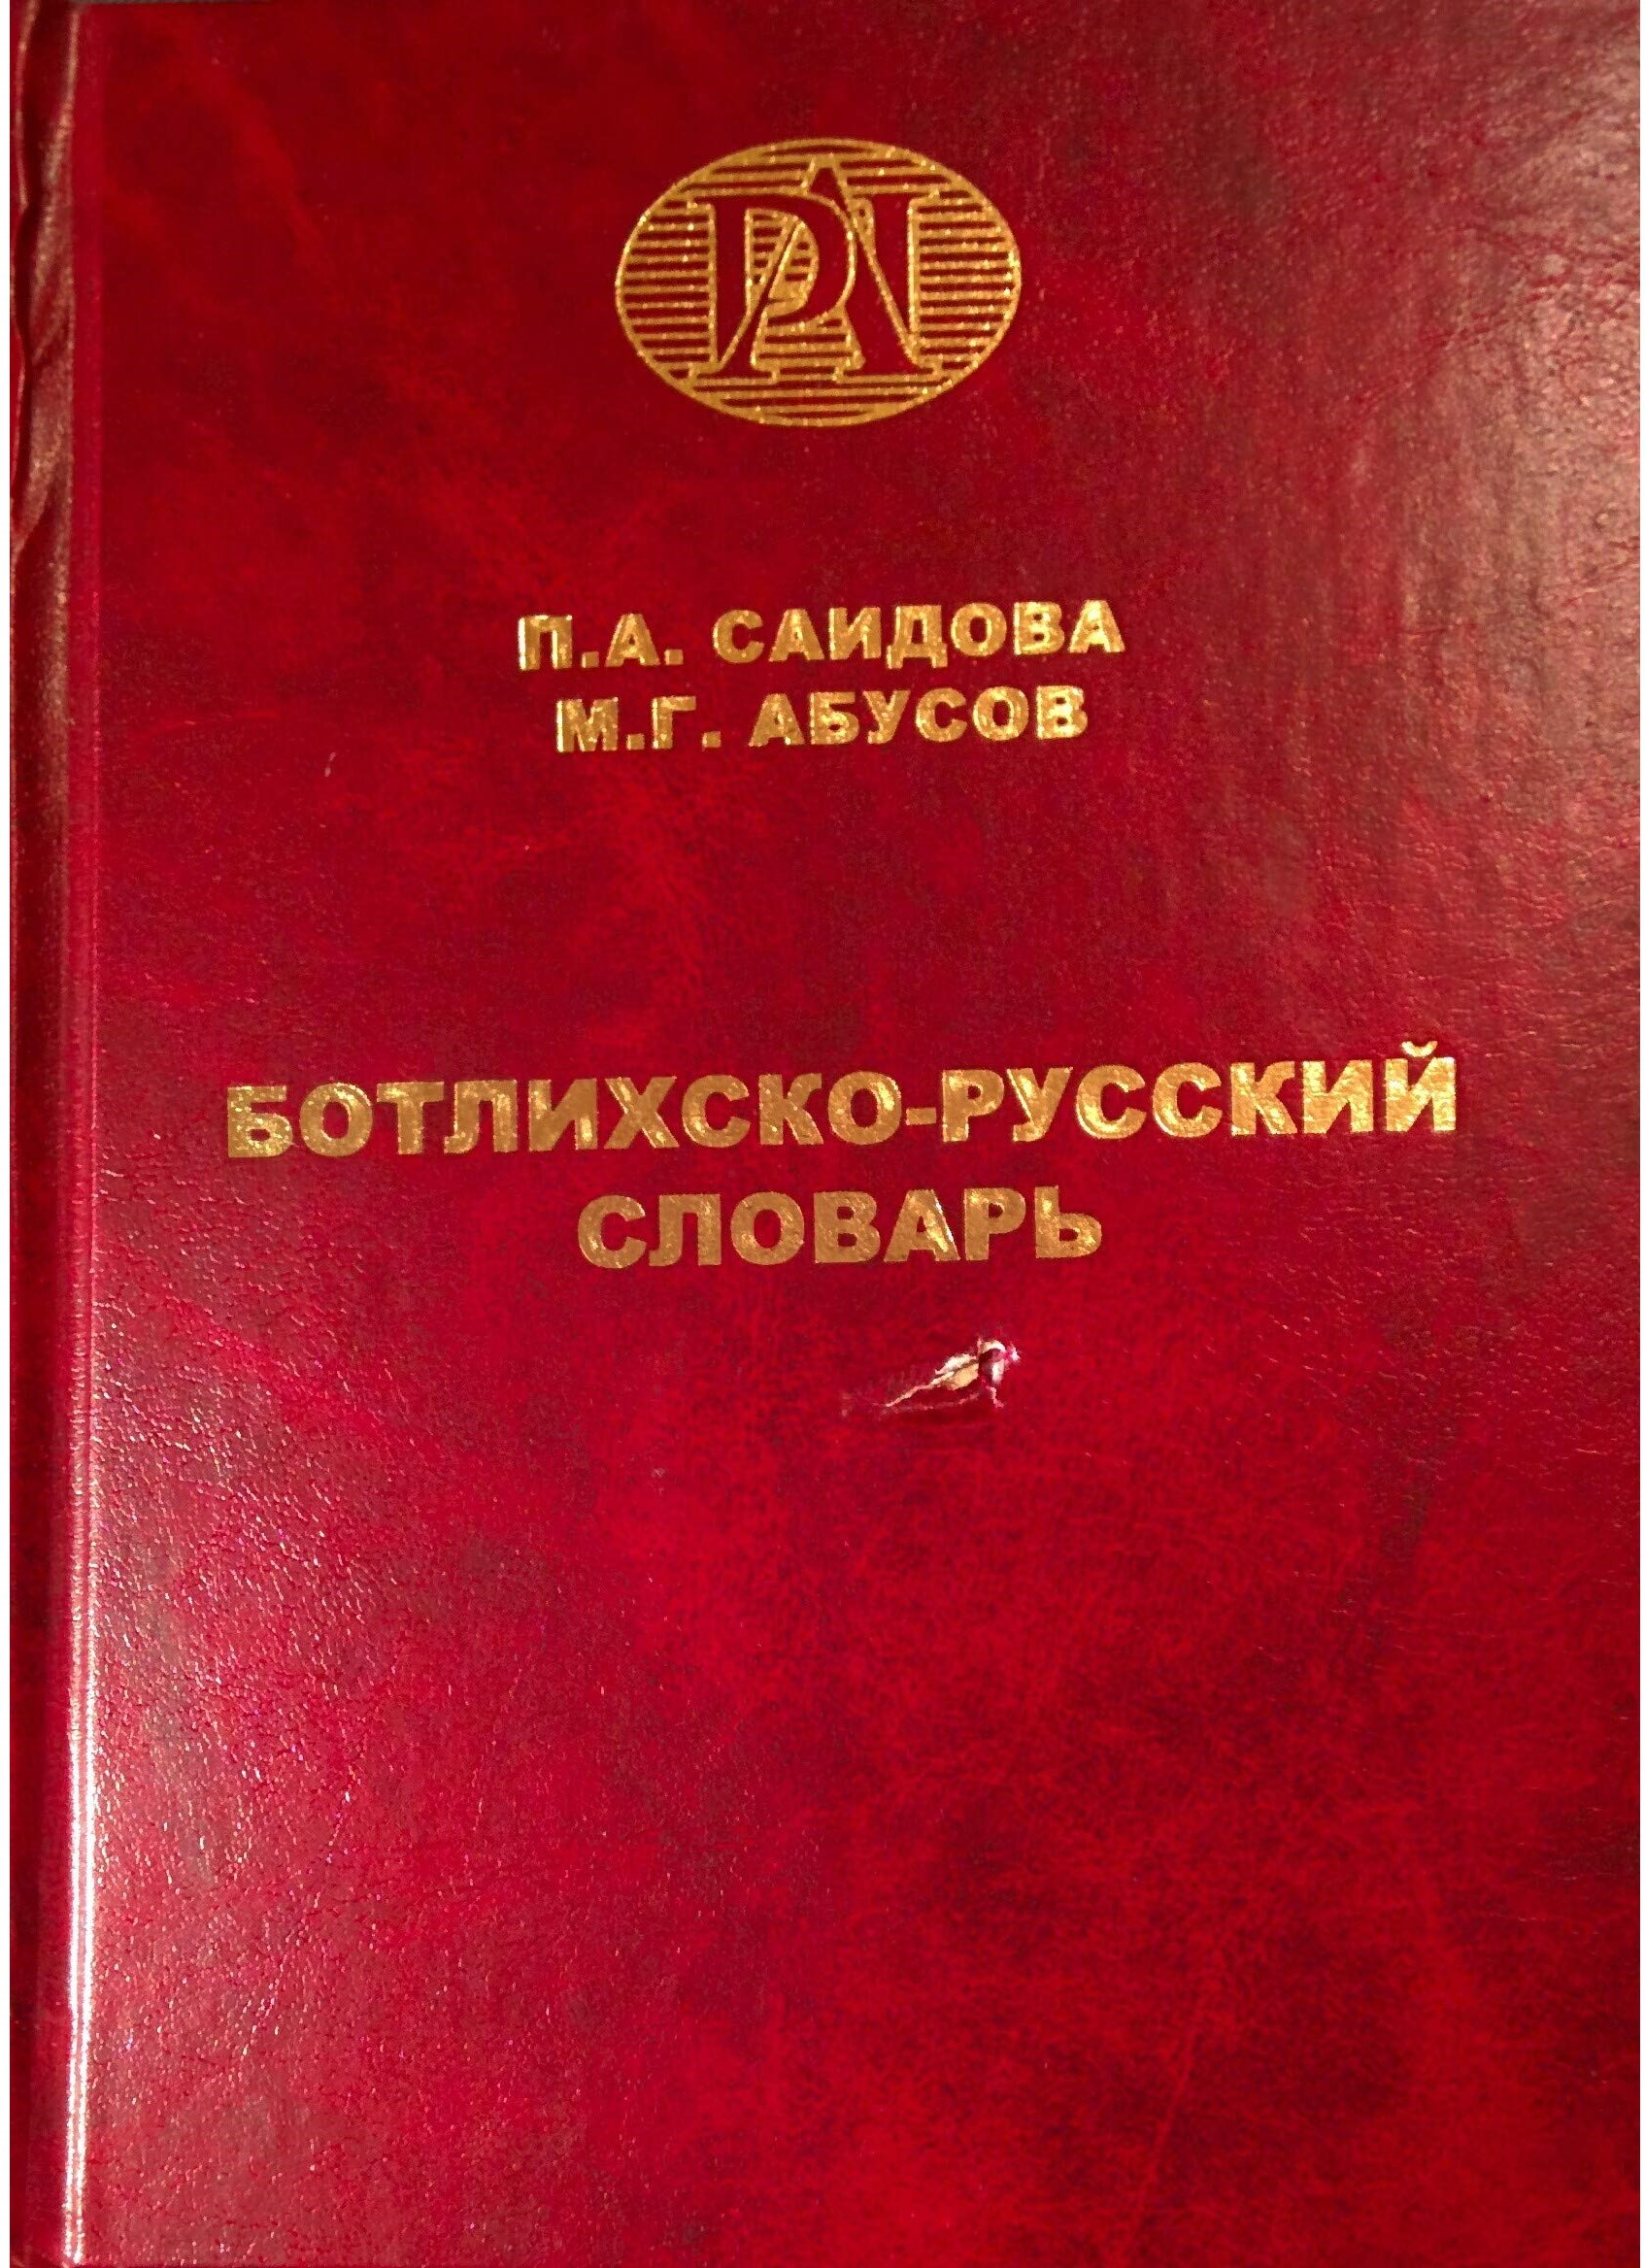
\includegraphics[height=6cm]{images/abusov2012.jpg} 
\label{abusov2012}
\end{subfigure}
\begin{subfigure}
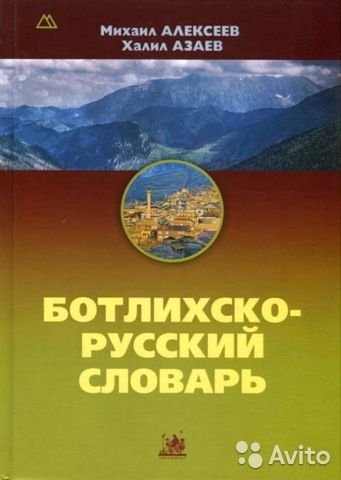
\includegraphics[height=6cm]{images/alekseev2019.jpg}
\label{alekseev2019}
\end{subfigure}
\caption{Two Botlikh-Russian dictionaries}
\label{two_dicts}
\end{figure}
\end{frame}

\begin{frame}{Two dictionaries}
\begin{itemize}
    \item \citep{saidovaabusov2012} compiled in the 2000s by a native speaker of Botlikh (Magomed G. Abusov) and an experienced linguist (Patimat A. Saidova)
    \item \citep{alekseev2019} compiled in the 1960s/1970s by a native speaker of Botlikh and philologist (Xalil G. Azaev), later (in the 2000s) systematized by an experienced linguist (Mixail E. Alekseev), and published posthumously after the editing by Timur A. Maisak
\end{itemize}
\end{frame}

\begin{frame}{Two dictionaries}
\begin{itemize}
    \item Comparable both quantitatively and qualitatively
    \item \textasciitilde{}8,000 headwords for \citep{saidovaabusov2012} vs. \textasciitilde{}9,000 words and expressions for \citep{alekseev2019}
    \item Although the data in \citep{alekseev2019} were collected several decades earlier, Magomed G. Abusov also consulted elderly speakers with the aim of collecting archaic vocabulary 
    \item \citep{saidovaabusov2012} also contains some notes on Miarso; reference to Miarso variants is not explicit in \citep{alekseev2019}, but it seems that such variants are occasionally reported in this dictionary too
    \item No metadata on the speakers consulted
    \item At first glance, the two resources seemed to display variation
\end{itemize}
\end{frame}

\begin{frame}{Our research}
\begin{itemize}
    \item Comparison of the two resources
    \item A unique opportunity to conduct a quantitative investigation of an understudied language
    \item Provide numerical approximations for the impressionistic observations available in the existing literature
    \item Analysis of both phonological and morphological features 
    \item Detect patterns of systematic variation within these two areas
\end{itemize}
\end{frame}

\begin{frame}{Outline}
\begin{itemize}
    \item Data 
    \begin{itemize}
        \item merging
        \item extracting grammatical information
        \item pairing and annotation
    \end{itemize}
    \item Analysis
    \begin{itemize}
        \item phonology (George Moroz)
        \item nominal morphology (Chiara Naccarato)
        \item verbal morphology (Samira Verhees)
    \end{itemize}
    \item Results and discussion
    \item Methodological remarks 
\end{itemize}
\end{frame}

\section{Data}
\begin{frame}{Merging}
From two .doc files to one .xls through a painstaking process of unification (George Moroz)
\begin{figure}[h]
\centering
\fbox{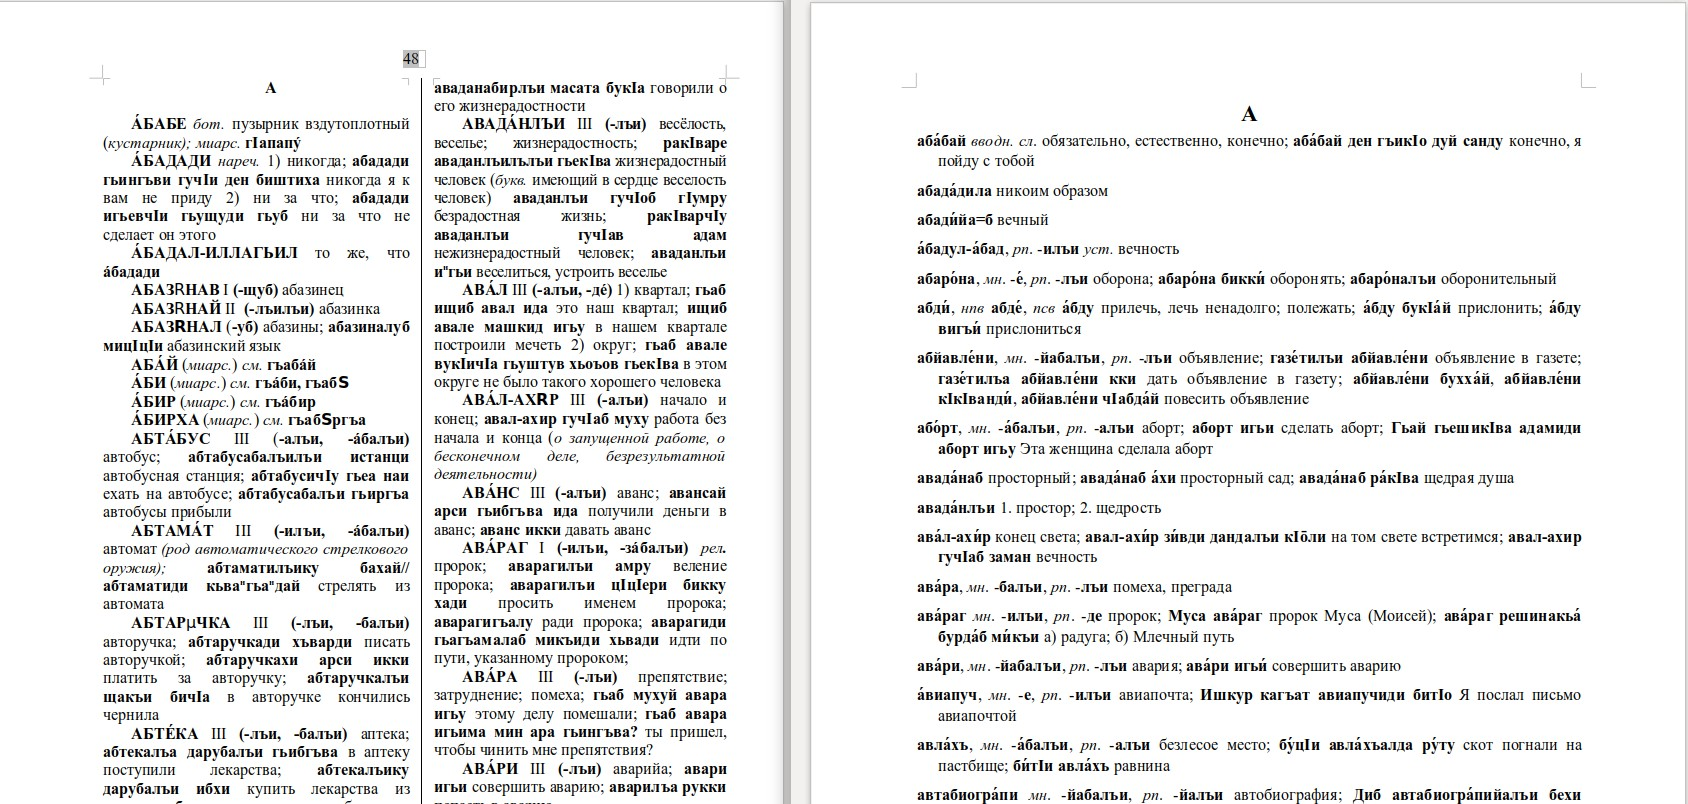
\includegraphics[scale=0.17]{images/dicts.jpg}}
\caption{Merging the dictionaries}
\end{figure}
\end{frame}

\begin{frame}{Extracting grammatical information}
\begin{itemize}
    \item Total number of lexemes extracted: 8,464 from \citep{saidovaabusov2012} and 6,821 from \citep{alekseev2019}
    \item Nouns: 2,871 from \citep{saidovaabusov2012} and 3,097 from \citep{alekseev2019}
    \begin{itemize}
        \item grammatical information: genitive and plural
    \end{itemize}
    \item Verbs: 1,504 from \citep{saidovaabusov2012} and 1,640 from \citep{alekseev2019}
    \begin{itemize}
        \item grammatical information: habitual and aorist
    \end{itemize}
\end{itemize}
\end{frame}

\begin{frame}{Extracting grammatical information}
\begin{figure}[h]
\centering
\fbox{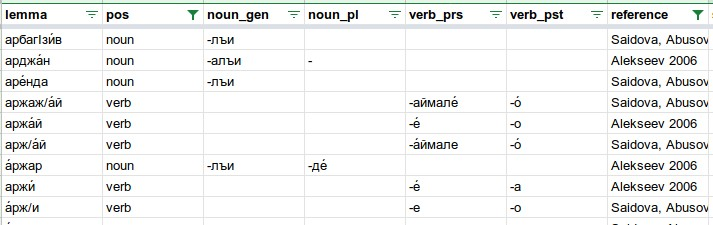
\includegraphics[scale=0.4]{images/table.jpg}}
\caption{The database}
\end{figure}
\end{frame}

\begin{frame}{Pairing}
\begin{itemize}
    \item We manually checked for lexemes represented in both dictionaries to carry out phonological and morphological analysis 
    % Here we could show Garik's Eulero Venn diagram, but we should check the numbers because I have the impression that we made quite a mess in our database  
\end{itemize}
\end{frame}

\begin{frame}{Annotation}
\begin{itemize}
    \item Manual correction of automatically extracted information about grammatical features
    \item Addition of further annotation (for features that appeared to be potentially relevant for our research):
    \begin{itemize}
        \item masdars
        \item borrowings
    \end{itemize}
\end{itemize}
    
\end{frame}

\section{Phonology}
\begin{frame}{Phonology}
    % Garik's research
\end{frame}

\section{Nominal morphology}
\begin{frame}{Nominal morphology}
Two topics investigated:
\begin{itemize}
    \item Formation of the plural
    \begin{itemize}
        \item to check the productivity of different suffixes
    \end{itemize}
    \item Formation of the genitive
    \begin{itemize}
        \item to study alternations in the formation of oblique stems
    \end{itemize}
\end{itemize}
Comparison of the two resources to look for possible variation in such areas of nominal morphology \\ (based on 1,072 pairs retrieved during the first annotation round)
\end{frame}

\begin{frame}{Plural formation in Botlikh}
\begin{itemize}
    \item A suffix is attached to the absolutive stem: \\ \textit{na} `thing' < \textit{na-\textbf{baɬi}} `things'
    \item With stems ending in a consonant, the vowel \textit{-a-} is often inserted before the suffix: \\ \textit{majmalak}  `monkey' < \textit{majmalak-\textbf{a}-\textbf{baɬi}} `monkeys'
    \item With stems ending in a vowel, alternation can occur: \\ \textit{ruš\textbf{a}}  `tree' < \textit{ruš\textbf{i}-\textbf{baɬi}} `trees', \\ \textit{sal\textbf{u}}  `tooth' < \textit{sal\textbf{a}-\textbf{baɬi}} `teeth', \\ \textit{buraɬ\textbf{i}}  `pitcher' < \textit{buraɬ\textbf{a}-\textbf{baɬi}} `pitchers'
\end{itemize}
\end{frame}

\begin{frame}{Plural formation in Botlikh}
Among the most common suffixes are:
\begin{itemize}
    \item \textit{-baɬi} and allomorphs (\textit{-maɬi} for stems ending in a nasal, \textit{-wabaɬi} for stems ending in -\textit{u}, etc.), the variant \textit{-zabaɬi} (mostly with borrowings) \\ \textit{apicer} `officer' < \textit{apicer-\textbf{zabaɬi}} `officers'  
    \item \textit{-de} (mostly for stems ending in a sonorant) \\ \textit{ambur} `roof' < \textit{ambur-\textbf{de}} `roofs'
    \item \textit{-e} and its variant \textit{-we} (for stems ending in -\textit{u}) \\ \textit{čan} `deer' < \textit{čan-\textbf{e}} `deers'
\end{itemize}
Other, less common, suffixes are: -\textit{(b)daɬi}, -\textit{(b)diɬi}, -\textit{(a)l}, -\textit{rdi}, -\textit{bala(l)}
\end{frame}

\begin{frame}{Plural formation in Botlikh}
\centering
Can our dictionary data help us be more precise about the distribution/frequency/productivity of plural suffixes in Botlikh? \\ ... \\ Do the two dictionaries show any variation in these respects?
\end{frame}

\begin{frame}{Plural suffixes in the dictionaries}
\begin{itemize}
    \item Plural suffixes are not reported for all nouns, cf. \textit{singularia tantum} and plural entries (nationalities, \textit{pluralia tantum})
    \item Quite often more than one variant is reported
\end{itemize}
\begin{table}[]
\caption{Plural suffixes in the dictionaries}
\centering
\begin{tabular}{lcc}
          & \multicolumn{1}{l}{\textbf{Saidova \& Abusov (2012)}} & \multicolumn{1}{l}{\textbf{Alekseev \& Azaev (2019)}} \\
\textbf{-\textit{(x)baɬi}}  & 292                                          & 298                                          \\
\textbf{-\textit{de}}       & 128                                          & 354                                          \\
\textbf{-\textit{(w)e}}     & 141                                          & 239                                          \\
\textbf{other}     & 24                                           & 21                                           \\
\textbf{no plural} & 499                                          & 193                                         
\end{tabular}
\end{table}
\end{frame}

\begin{frame}{Plural suffixes in the dictionaries}
    
\end{frame}

\section{Verbal morphology}
\begin{frame}{Verbal morphology}
    
\end{frame}

\section{Discussion}
\begin{frame}{Discussion}
    
\end{frame}

\section{Methodological remarks}
\begin{frame}{Methodological remarks}
    
\end{frame}

\section{The end}
\begin{frame}{The end}
\begin{figure}[h]
\centering
\fbox{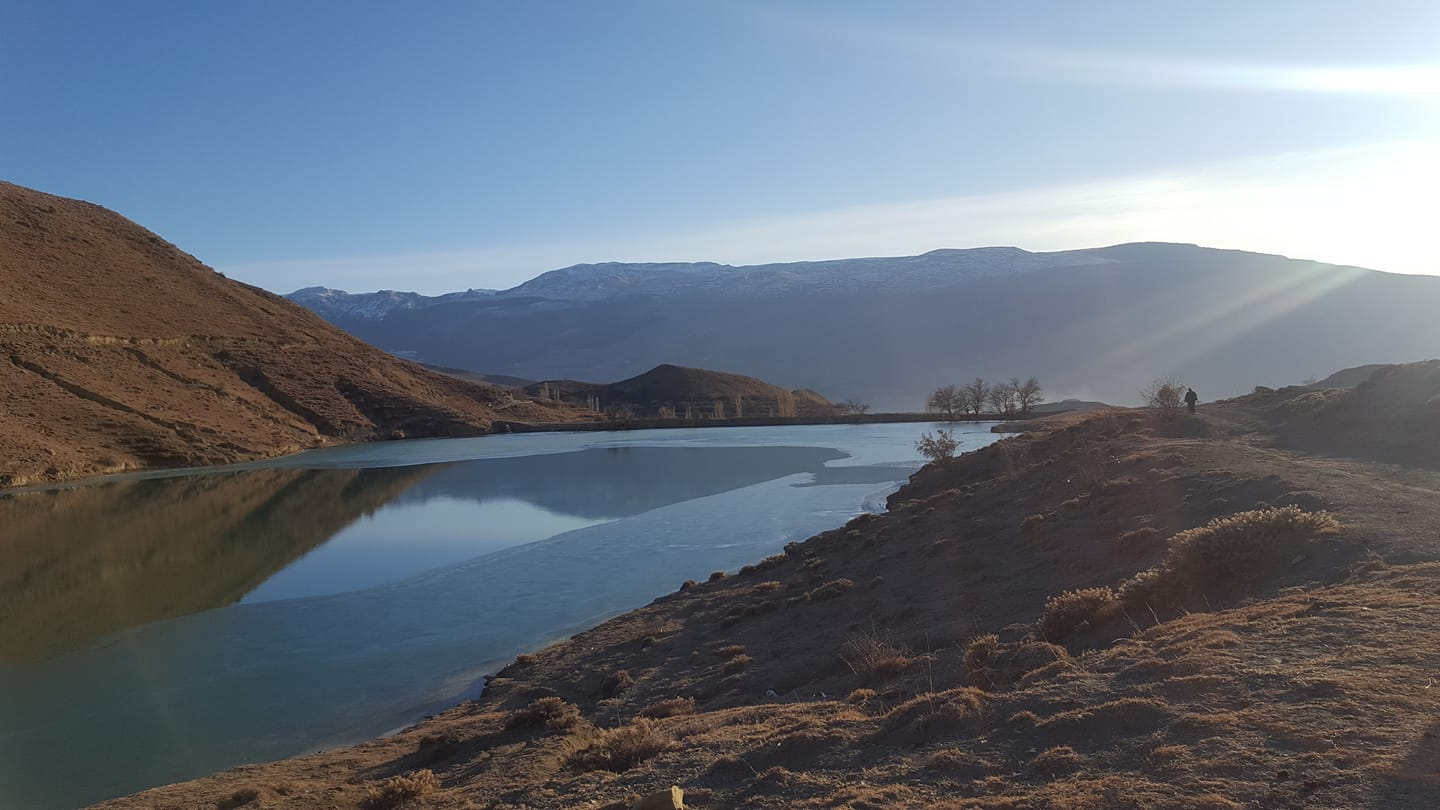
\includegraphics[height=6cm]{images/arqule.jpg}}
\end{figure}
\end{frame}

\section{Abbreviations}
\begin{frame}{Abbreviations}
\tiny{\printglossary}
\end{frame}

\section{References}
\begin{frame}[allowframebreaks]{References}
\printbibliography
\end{frame}

\end{document}